\documentclass[letterpaper,12pt]{article}
\usepackage[utf8]{inputenc}

\usepackage{rotating}
\usepackage[top=1in, bottom=1in, left=1in, right=1in]{geometry}
\usepackage{graphicx}
\usepackage[numbers,square,sort&compress]{natbib}
\usepackage{setspace}
\usepackage[cdot,mediumqspace,]{SIunits}
\usepackage{hyperref}
\usepackage{mathtools}
\usepackage{url}
\usepackage{authblk}
\usepackage{placeins}
\usepackage{float}

\onehalfspacing
\title{Functional Analysis: Interpolation}
\author{Anita Bahmanyar}
\affil{\small {Student Number: 998909098}}
\affil{\small {anita.bahmanyar@mail.utoronto.ca}}
\date{December 19, 2014}

\usepackage{graphicx}

\renewcommand\thesubsection{\alph{subsection}}

\begin{document}

\maketitle

\section{Introduction}
In physics we are often given a few data points by sampling or experimenting and we need to estimate the values of our model between these points. The method commonly used to solve this problem in numerical analysis is interpolation. This is only an estimation so it introduces error to our calculation. Interpolation is passing a curve from all the data points. There is one other case where interpolation becomes handy. For instance, we have a very complicated function to evaluate and if we want to evaluate it at all the desired points it would take a long time to compute it and it is not efficient. In that case, we can take advantage of interpolation to estimate the value of the function at the points we want given the value of the function at only a few points. This estimation for such a complex function might not be very accurate but the amount of computational time we save is worth the accuracy we lose.

\section{Interpolation Types}
\subsection{Linear Interpolation}
Linear interpolation is the simplest way of getting the values of a function in between points. Linear interpolation is a method to fit a curve to the points using linear functions. If we know the coordinates of two points as $A=(x_0,y_0)$ and $B=(x_1,y_1)$, the linear interpolation between these two points would simply be a straight line. Figure 1 shows the schematic view of linear interpolation.

%figure 1
\FloatBarrier
\begin{figure}[H]
\centering
\includegraphics[scale=0.5]{linear_plot.png}
\caption{We can calculate the value of $C=(x_2,y_2)$ using linear interpolation knowing the coordinates of $A=(x_0,y_0)$ and $B=(x_1,y_1)$.}
\end{figure}
\FloatBarrier


\subsubsection{Mathematical Approach}



The equation of a straight line is given by:
\begin{equation}
y = y_0 +\frac{(x-x_0)(y_1-y_0)}{x_1-x_0}
\end{equation}
where $\frac{y_1-y_0}{x_1-x_0}$ is the slope of the line. Therefore, having the values of the points A and B, we can compute the value of $y_2$ given the value of $x_2$.
This can be considered as the weighted average. The weights are inversely related to the distance from the end points to the unknown point; the closer point has more influence than the farther point. 
Since this method only returns equation of lines in between each two points, the more the number of points available, the better the interpolation would be.
The points are simply joined by straight line segments resulting in discontinuities at each point. 

\subsubsection{Example}
\textbf{Code: linear.py}
\\Figure 2 shows the $\sin(x)$ function and the interpolated curves using 10 knots using my linear interpolation code and scipy 1d linear interpolation. Both interpolations are almost the same showing that my code is as good as scipy. The more knots we add, the better the interpolated values demonstrate the sin function. Figure 3 shows the same curves as figure 2 with 20 knots. We can see that the interpolated values are getting closer to the $\sin(x)$ function.




%figure 2
\FloatBarrier
\begin{figure}[H]
\centering
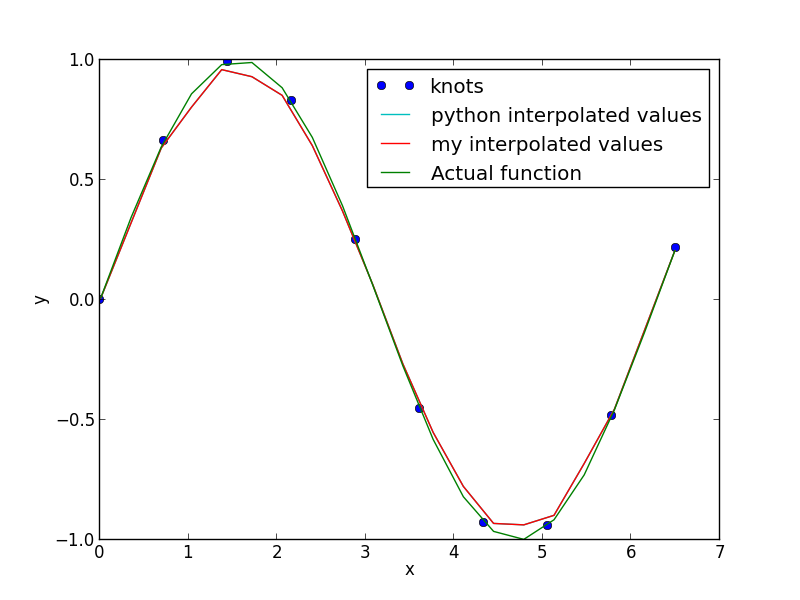
\includegraphics[scale=0.5]{lin_sin.png}
\caption{The interpolated values from my code and scipy module are very similar that they go on top of one another. This is generated using 10 knots.}
\end{figure}
\FloatBarrier

%figure 3
\FloatBarrier
\begin{figure}[H]
\centering
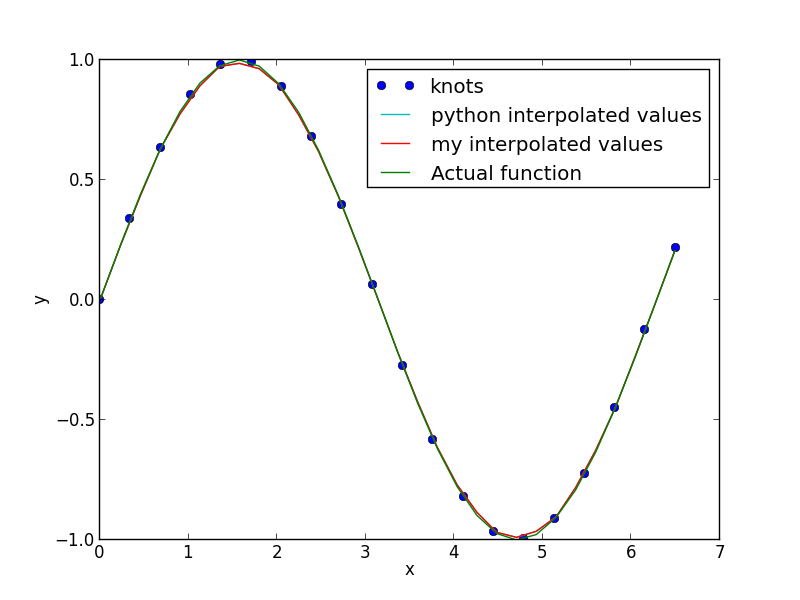
\includegraphics[scale=0.5]{lin_sin_morepoints.png}
\caption{The interpolated values from my code and scipy module are very similar that they go on top of one another. This is similar to previous figure except this is with more knots. This has 20 knots compared to 10 in the previous figure. We can see that the interpolated curves are getting closer to the function.}
\end{figure}
\FloatBarrier
The interpolated values using Scipy linear 1d interpolation is very similar to the values I got from my linear interpolation code.The mean value of the difference between the Python linear interpolation and my interpolation method is $\sim 1.735 \times 10^{-17}$. Linear interpolation just gives us an overall shape of the function, it is not very accurate since it only uses straight lines between each points, so it would not be a smooth function. However, as we add more knots it would seem smoother and more similar to the actual function.


\subsubsection{Error Analysis}
The error on linear interpolation is of order of $O(h^2)$, which means the error is proportional to the square of the distance between the data points. It has the form of:
\begin{equation}
f(x)-P_1(x) = \frac{(x-x_0)(x-x_1)}{2}f''(c_x)
\end{equation}
where $P_1(x)$ is the interpolation function in the interval $[a,b]$ and $c_x$ is a point in this interval.  This can be obtained writing $f(a)$ and $f(b)$ as their Taylor series approximation and writing $P(x) = \frac{(x-x_1)}{x_0-x_1}f(x_0) + \frac{(x-x_0)}{(x_1-x_0)}f(x_1)$. Then we can substitute for $f(a)$ and $f(b)$ in $P(x)$ and get the following:
\begin{equation}
f(x)-P_1(x) = \frac{1}{2}(x-b)(x-a)f''(x)+...
\end{equation}
To give a rough estimate of the error in the $\sin(x)$ function using 20 knots and 30 points in between the knots, we get the following values for the first two knots and a point in between:
\\$a=0$
\\$b=0.34210526$
\\$u_x=0.23344828$
\\$|f(x)-P_1(x)| = |\frac{1}{2} (0.23344828-0) (0.23344828-0.34210526) (-\sin(0.23344828)) |$
\\Therefore, the error would be $\sim 0.003$

\subsection{Cubic Spline Interpolation}
Cubic spline interpolation is a more accurate and advanced way of fitting a curve to data points than the linear interpolation. We need to make sure the piecewise curves passing through the points have continuous second derivative at the knots. For this purpose, we need to use polynomials that are of order 3 or higher and that is where the name cubic comes from.
\subsubsection{Mathematical Approach}
The aim is to fit a curve passing through points $(x_i,y_i)$ where $i=0,1,...,n$, so we interpolate between points $(x_{i-1},y_{i-1})$ and $(x_i,y_i)$ with polynomials $y_i = q_i(x)$.


Splines take a shape so that to minimize the bending of the curve between each two knots. We require the following conditions:
\begin{equation}
q'_i(x_i) = q'_{i+1}(x_i) 
\end{equation}

\begin{equation}
q''_i(x_i) = q''_{i+1}(x_i) 
\end{equation}
for all i, $1\leq i \leq n-1$.

%equation
\begin{equation}
\frac{k_{i-1}}{x_i - x_{i-1}} +    \left (    \frac{1}{x_i - x_{i-1}} + \frac{1}{x_{i+1}-x_i} \right ) 2k_i + \frac{k_{i+1}}{x_{i+1}-x_i} = 3  \left(  \frac{y_i - y_{i-1}}{(x_i - x_{i-1})^2} + \frac{y_{i+1}-y_i}{( x_{i+1}-x_i )^2} \right)
\end{equation}
for $i=1,2,...,n-1$. This gives us $n-1$ equations including $k_0$, $k_1$, ..., $k_n$.

For the two knots at both ends, the condition is different and we have:
%equation
\begin{equation}
\frac{2}{x_1-x_0}k_0 + \frac{1}{x_1-x_0}k_1 = 3\frac{y_1-y_0}{(x_1-x_0)^2}
\end{equation}


%equation
\begin{equation}
\frac{1}{x_n-x_{n-1}}k_{n-1} + \frac{2}{x_n-x_{n-1}}k_n = 3\frac{y_n-y_{n-1}}{(x_n-x_{n-1})^2}
\end{equation}

Equations 7 and 8 give us two more equations which along with the previous $n-1$ equations from 6 we would have $n+1$ equations to solve for $k_0$,$k_1$,..,$k_n$ values. The cubic spline�s coefficients can be found by solving a tridiagonal linear system:
%equation, matrix form
\begin{equation}
\begin{bmatrix}
a_{11} & a_{12} & &  &  & &\\ 
a_{21} & a_{22} & a_{23} & &  & &\\ 
 & a_{31} & a_{32} & a_{33} & & &\\
 &  & \ddots & \ddots & \ddots& &\\ 
 &  & & a_{n-1n-2}& a_{n-1n-1}&a_{n-1n}\\ 
 &  & & & a_{nn-1} & a_{nn}  
\end{bmatrix}
\begin{bmatrix}
k_0\\ 
k_1\\ 
k_2\\ 
\vdots\\ 
k_{n-1}\\
k_n\\
\end{bmatrix} = 
\begin{bmatrix}
b_0\\ 
b_1\\ 
b_2\\ 
\vdots\\ 
b_{n-1}\\
b_n \\
\end{bmatrix}
\end{equation}

Then having the values of $k_i$, we can calculate $a_i$ and $b_i$ values:
%equation
\begin{equation}
a_i = k_{i-1} (x_i-x_{i-1}) - (y_i - y_{i-1})
\end{equation}

%equation
\begin{equation}
b_i = -k_i (x_i - x_{i-1}) + (y_i - y_{i-1})
\end{equation}
and use these values to calculate $q_i$ values:

%equation
\begin{equation}
q_i = (1-t)y_{i_1} + ty_i + t(1-t) (a_i (1-t) +b_it)
\end{equation}
where t is:

%equation
\begin{equation}
t = \frac{x-x_{i-1}}{x_i - x_{i-1}}
\end{equation}

This will give us a function $q$ for the points between each two knots, so we will have $n$ different functions for the $n+1$ knots.

\subsubsection{Example}
\textbf{Code:cubic\_spline.py}
\\Figure  4 shows a prime example of using my cubic spline code to get the values using only 5 arbitrary knots.

%figure 4, arbitrary cubic interpolation
\FloatBarrier
\begin{figure}[H]
\centering
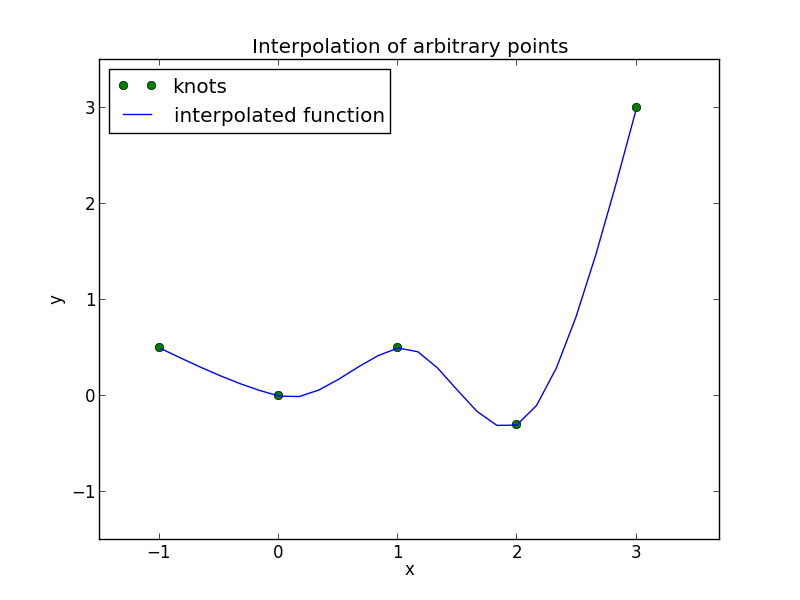
\includegraphics[scale=0.5]{interp_arbitrary.png}
\caption{Interpolation of 5 arbitrary points using my code for cubic spline interpolation.}
\end{figure}
\FloatBarrier
Figure 5 shows the $\sin(x)$ function and its cubic interpolated values. As you can see, the Python built-in interpolation function does a better job in cubic spline interpolation than my code. The zoomed in figure shows that my interpolation is still very close to the actual function even though it differs a bit from the function and the python interpolated function.


%figure 5
\FloatBarrier
\begin{figure}[H]
\centering
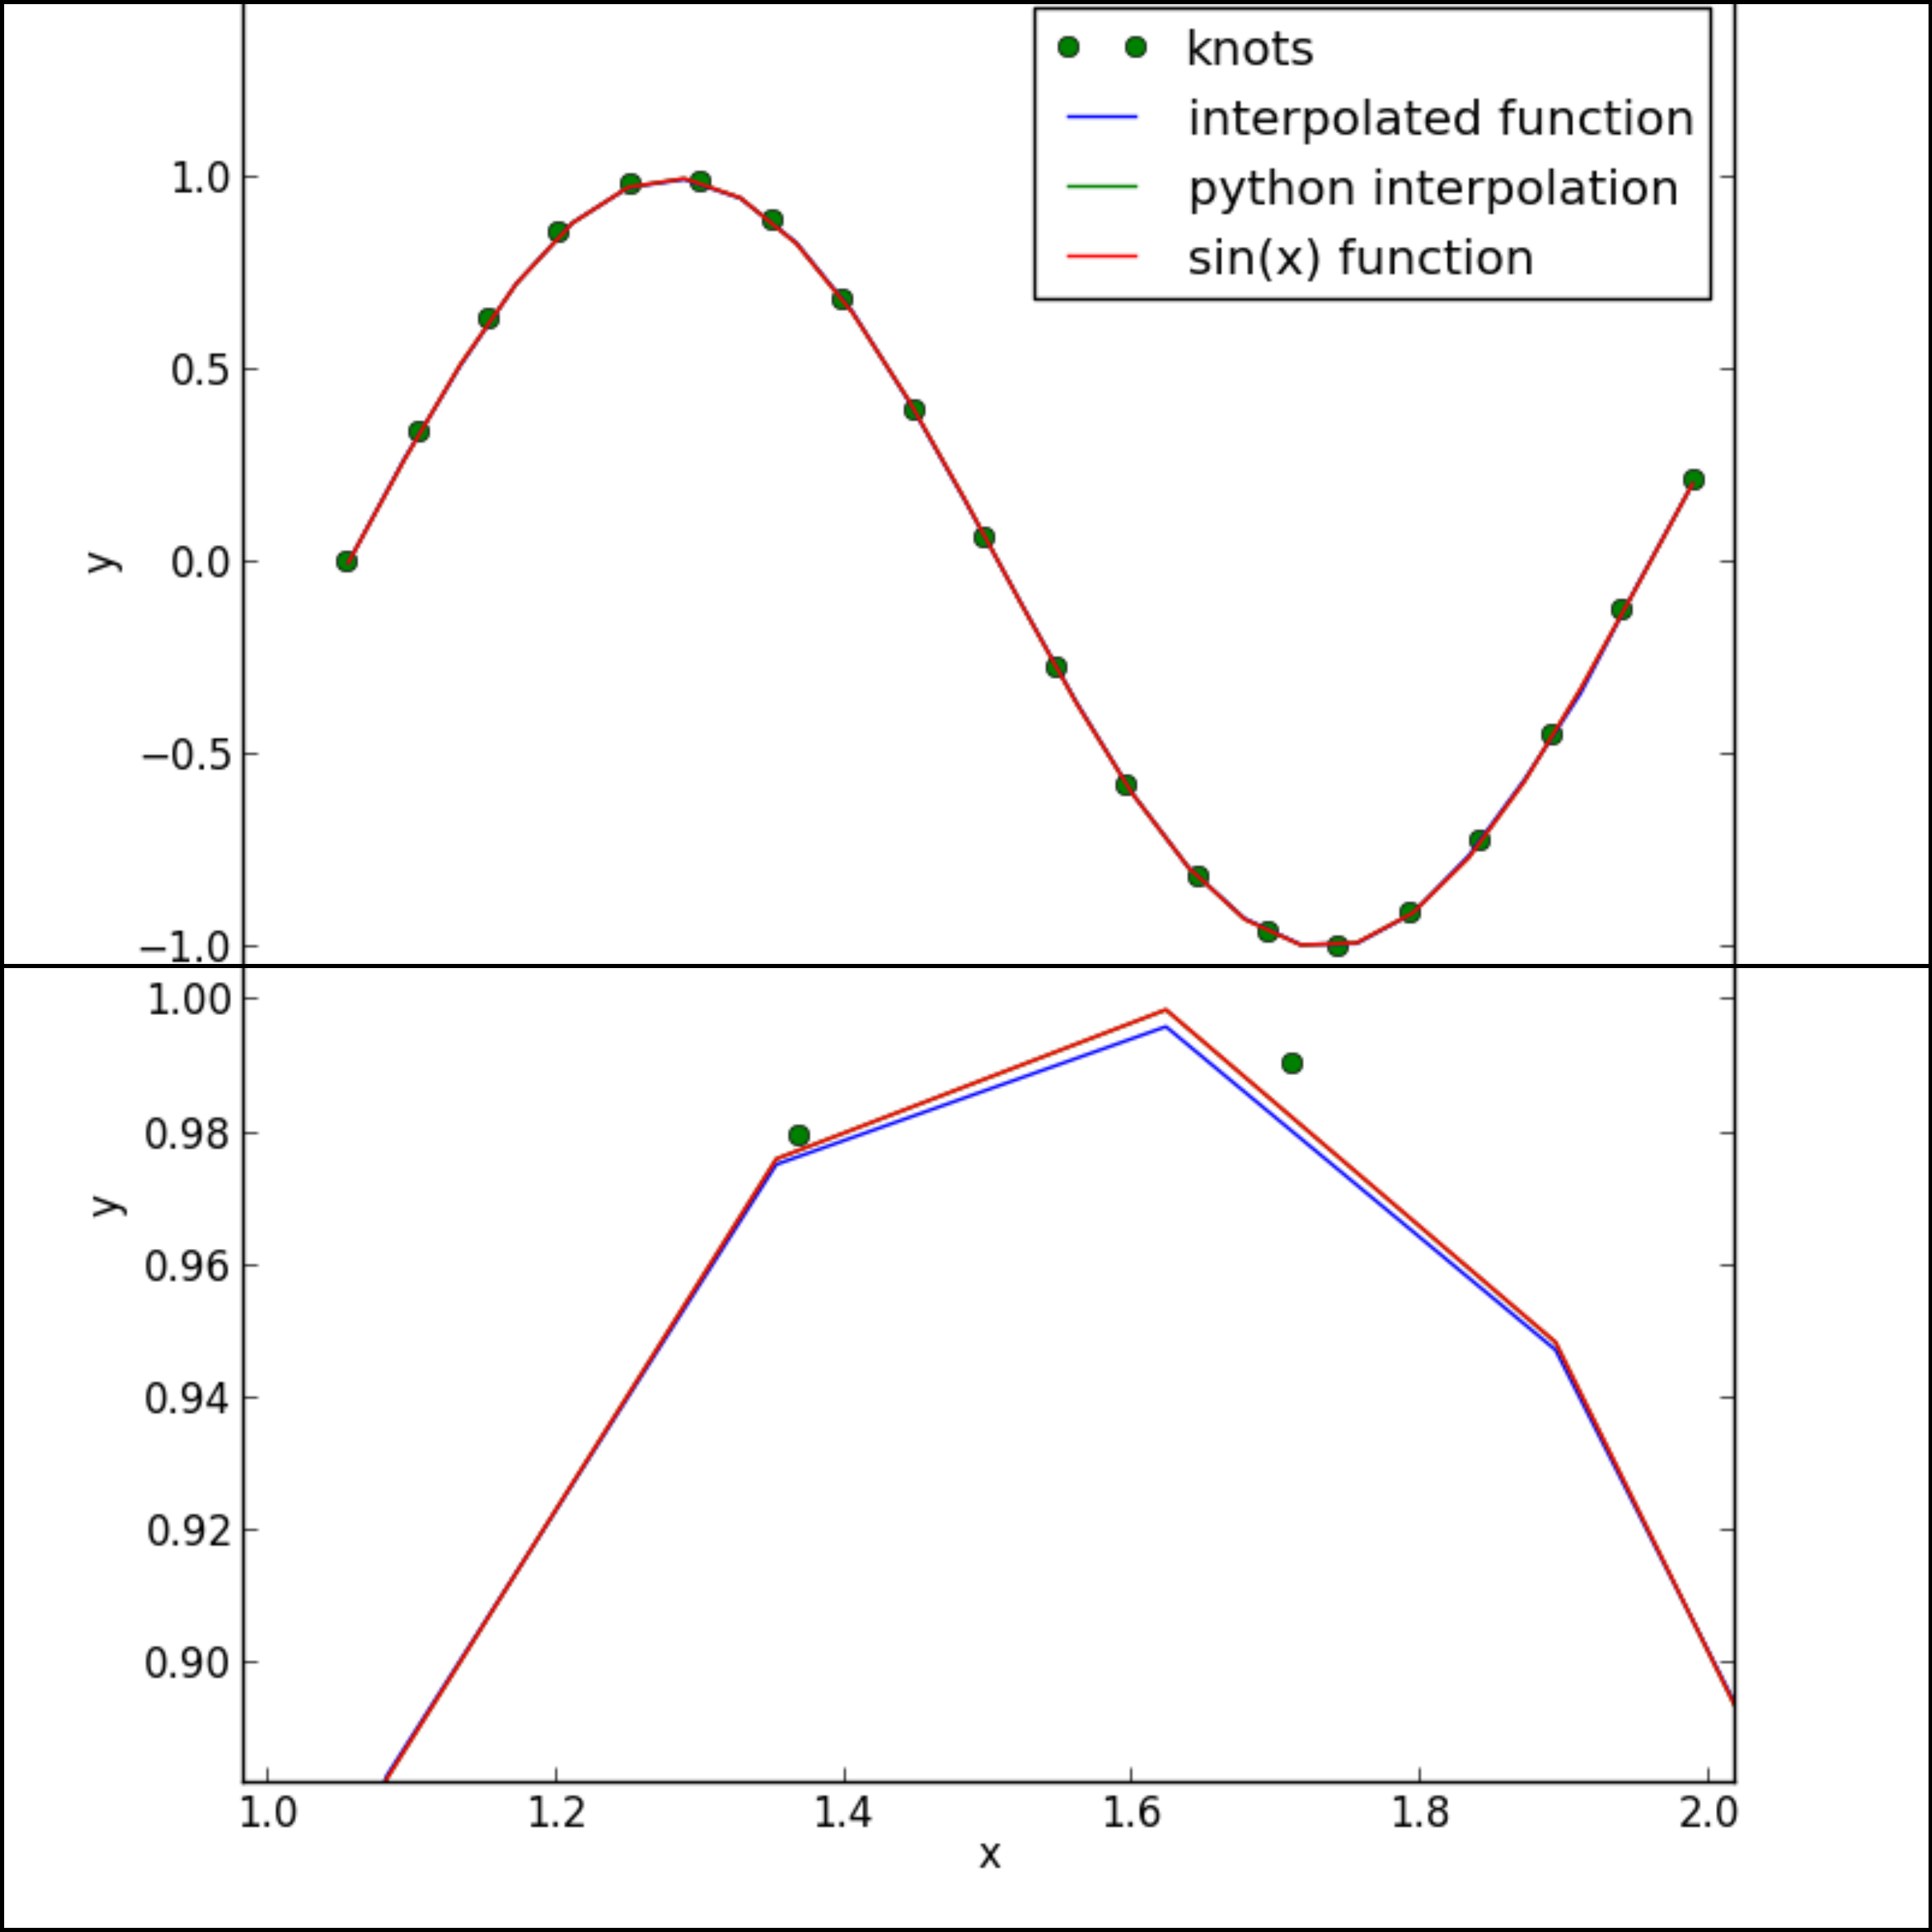
\includegraphics[scale=0.09]{cubic_compared_final.png}
\caption{Upper: Knots are shown in green dots, red is the actual sin(x) function and blue and green are my interpolated function and Python built-in interpolation function, respectively. Lower: Zoomed in version of the figure above. Python built-in function does a better job in cubic spline interpolation than my code.}
\end{figure}
\FloatBarrier

%difference plot
\FloatBarrier
\begin{figure}[H]
\centering
\includegraphics[scale=0.5]{difference_less.png}
\caption{Difference between my cubic spline interpolated values and scipy cubic interpolated values. The values are very small showing that my code works fine.}
\end{figure}
\FloatBarrier

\subsubsection{Error Analysis}
The error in cubic spline interpolation is of order $O(h^4)$. The error would be the maximum difference between the value of the function we are approximating and our interpolated value. The error is given by:
\begin{equation}
\left | s-f \right | \sim \frac{5}{384}. \left | f^{(4)} \right |. h^4
\end{equation}
where $|s-f|$ is the difference between interpolated and the function value, $f^{(4)}$ is the value of fourth derivative of the function and h is the spacing between knots.
For example, if we do the interpolation on the function $y(x) = \sin(x)$ over the interval [0,3] with $h$= 0.1, what would the error be?

\\We know $f^{(4)}(x)$ = $\sin(x)$; therefore, $f^{(4)}(x) \leq$ 1. So the value of the error would be:
\\ $\frac{5}{384}.1.(0.1)^4$ $\approx$ $\frac{1}{768000} \approx 1.3 \times 10^{-6}$. This error is very small so the cubic spline interpolation is a good approximation of the function. 

Now to see how accurate my code is, I have applied the code to do the interpolation for the function $\sin(x)$ in the interval [0,6.5] with 20 points, so $h$ = 0.325 here. So the error would be $\sim 1.46 \times 10^{-4}$. This is still quite a small error.

\subsection{Bilinear Interpolation}
Bilinear interpolation is the same as linear interpolation which is extended into two dimensions. Unlike 1D interpolation where you entered $x$ values and got $y=f(x)$ values out, this would require you to enter $x$ and $y$ values to get the value of the function $z = f(x,y)$ out. Figure 7 shows a schematic view of bilinear interpolation.

%figure 5
\FloatBarrier
\begin{figure}[H]
\centering
\includegraphics[scale=0.5]{bilinear_plot.png}
\caption{The red points show the knots and point P, shown in green, is where we want to calculate the value. }
\end{figure}
\FloatBarrier


\subsubsection{Mathematical Approach}
The four points indicated by red dots in figure 7 have the values of:
\\$Q_{11} = (x_1,y_1)$, $Q_{12} = (x_1,y_2)$, $Q_{21} = (x_2,y_1)$ and $Q_{22} = (x_2,y_2)$. Also, the blue dots in figure 6 are $R_1=(x,y_1)$ and $R_2=(x,y_2)$. The green dot is the point where we want to find the value, $P=(x,y)$.
\\Doing linear interpolation in x-direction first would give us:
\begin{equation}
f(R_1) \approx \frac{x_2-x}{x_2-x_1}f(Q_{11}) + \frac{x-x_1}{x_2-x_1}f(Q_{21})
\end{equation}
and
\begin{equation}
f(R_2) \approx  \frac{x_2-x}{x_2-x_1}f(Q_{12}) + \frac{x-x_1}{x_2-x_1}f(Q_{22})
\end{equation}
Then we continue the interpolation in y direction which gives us:
\begin{equation}
f(P) \approx \frac{y_2-y}{y_2-y_1}f(R_1) + \frac{y-y_!}{y_2-y_1}f(R_2)
\end{equation}
Finally, the estimate of the interpolated function would be:
\begin{eqnarray}
f(x,y) \approx \frac{1}{(x_2-x_1)(y_2-y_1)} \left ( f(Q_{11})(x_2-x)(y_2-y) + 
\\f(Q_{21})(x-x_1)(y_2-y) + 
\\f(Q_{12})(x_2-x)(y-y_1) + 
\\f(Q_{22})(x-x_1)(y-y_1) )\right)
\end{eqnarray}
This could have been done by doing the linear interpolation first in y direction and then in x direction without any change in the result. This kind of interpolation is linear in x and in y direction separately but not as a whole despite its name. Figure 8 shows how bilinear interpolation method works. We multiply the area of each square by the value of the knot on the opposite side and divide the result by the area of the whole square ABCD to normalize the values.

%figure of colours
\FloatBarrier
\begin{figure}[H]
\centering
\includegraphics[scale=0.5]{bilinear_plot2.png}
\caption{The value of the function at point $P=(x,y)$ is the sum of the value of each coloured point multiplied by the area of the same colour divided by the area of ABCD rectangle to normalize it.}
\end{figure}
\FloatBarrier

\subsubsection{Example}
\textbf{Code:bilinear.py}
\\Figure 9 shows an example of running my code for bilinear interpolation. The four points given are located at the sides of a unit square and the $Q_{11}$, $Q_{12}$, $Q_{21}$ and $Q_{22}$ values are 0,1,1,0.5, respectively. I have compared the values I got for interpolation using my own code with the values from scipy 2d interpolation and the two plots seem very similar. The mean value of the absolute value of the difference between the values of the two is $\sim 1.998 \times 10^{-17}$.

%contour plot
\FloatBarrier
\begin{figure}[H]
\centering
\includegraphics[scale=0.4]{table1.png}
\caption{Comparison between my bilinear interpolation code and scipy 2d interpolation using four points on a unit square. Left: Using my code. Right: Using scipy. The two figures are quite similar showing my code works fine.}
\end{figure}
\FloatBarrier


\section{Analysis}
\textbf{Code: step\_function.py and exponential.py}
\\In this section, I will test my code for different functions and compare it with scipy interpolation modules. Figures 10 and 11 show the step function curve, its linear and cubic interpolation values using both my code and scipy module. The two plots show the same curves using 15 knots, 20 and 100 points in between, respectively. We can see that as we keep the number of knots the same and increase the number of points in between the knots, we get a better approximation of the step function. However, no matter how many points we add in between knots, there is always an effect at the edges called Gibb's phenomena which is due to the discontinuity of the step function. In the case of the step function linear interpolation does a better job both in the case of my code and scipy code and the scipy does a better job in cubic interpolation than my code.

\FloatBarrier
\begin{figure}[H]
\centering
\includegraphics[scale=0.5]{step201.png}
\caption{15 knots and 20 points in between.}
\end{figure}
\FloatBarrier

\FloatBarrier
\begin{figure}[H]
\centering
\includegraphics[scale=0.5]{step1001.png}
\caption{15 knots and 100 points in between.}
\end{figure}
\FloatBarrier

Figure 12 shows the function $e^{-4x^2}$ and the interpolated values. My cubic spline interpolation is not as good as scipy cubic interpolation, while both mine and scipy linear interpolation curves match up and are the same.

%exponential plot
\FloatBarrier
\begin{figure}[H]
\centering
\includegraphics[scale=0.45]{exponential.png}
\caption{$e^{4x^2}$ function along with linear and cubic spline interpolation using both my code and scipy. The linear interpolation using my code and scipy match up exactly while the cubic spline interpolations differ.}
\end{figure}
\FloatBarrier


\section{Conclusion}
Interpolation is a great tool in numerical analysis. It estimates the values of a function if we know the values of the function for only a few points. This introduces error to the calculations but the computation time it saves is worth loosing a bit of accuracy.
Cubic spline interpolation approximates the curve between data points much better than linear interpolation. The error in linear interpolation is of order two while the error in cubic spline interpolation is of order four. In one of the examples we saw that the error was 1000 times smaller in cubic spline method than the linear interpolation method.
Generalization of the error in polynomial interpolation:
\begin{equation}
f(x) - P_n(x) = \frac{(x-x_0)(x-x_1)...(x-x_n)}{(n+1)!}f^{(n+1)}(u_x)
\end{equation}
where $u_x$ is a point in the interval of interpolation.
\\My code for linear and bilinear interpolation has almost the same accuracy as the scipy 1d and 2d interpolation modules; however my cubic spline interpolation is a small bit different from that of the scipy. This difference is very small as shows in figure 6 and can be considered as good approximation of the curve. It does not work as well for step function and it might be due to the discontinuity problems of the step function that scipy is taking into account.


\section{References}
1-http://bmia.bmt.tue.nl/people/BRomeny/Courses/8C080/Interpolation.pdf
\\2-http://en.wikipedia.org/wiki/Linear\_interpolation
\\3-http://en.wikipedia.org/wiki/Bilinear\_interpolation
\\4-http://en.wikipedia.org/wiki/Spline\_interpolation
\\5-http://homepage.math.uiowa.edu/~atkinson/ftp/ENA\_Materials/Overheads/sec\_4-2.pdf
\\6-http://www-solar.mcs.st-andrews.ac.uk/~clare/Lectures/num-analysis/Numan\_chap3.pdf
\\7-http://en.wikipedia.org/wiki/Interpolation

\end{document}




